\documentclass{article}
\usepackage[utf8]{inputenc}
\usepackage{indentfirst} % to have indent in the first paragraphs
\usepackage{geometry}
\geometry{
    a4paper,
    left=30mm,
    right=30mm,
    top=20mm,
    bottom=25mm,
}
\renewcommand{\baselinestretch}{1.5}
\usepackage{times}
\usepackage{latexsym}
\usepackage{float}
\usepackage{graphicx}
\usepackage{microtype}
\usepackage{hyperref}
\usepackage{amssymb}
\usepackage{amsmath}
\usepackage[makeroom]{cancel}
\usepackage{import}
\usepackage{xcolor}
% \usepackage{tikz}

\usepackage[backend=biber, style=alphabetic, sorting=ynt]{biblatex}
\addbibresource{bibliography.bib}

\title{IN-STK5000 - Project 2a - Privacy analysis}
\author{Aurora Poggi, Fábio Rodrigues Pereira, Nick Walker \\
\emph{Project 9}}
\date{November 2021}

\begin{document}

\maketitle

\section{Introduction}
In this project, we model the effect of vaccination against Covid-19 on a population. Our goal is to design a vaccination strategy which minimizes the rate of deaths in the vaccinated population. 

\section{Adaptive Model Procedure}
\label{adaptive_procedure}

Our procedure begins by defining a "Trusted Curator" object in code. The Curator object provides a wrapper for the data which requires a user name and password to provide samples of the data. This is a layer of security for the data so that we can limit access to the population and vaccination information to researchers or other trusted parties who request access to the database. The data which is generated inside the Curator object (a population, from which we draw both features, actions, and outcomes, discussed later) is defined according to the simulator function provided in the Github repository\footnote{https://github.com/olethrosdc/ml-society-science/blob/master/src/covid/simulator.py}. 

After creating our Trusted Curator, we then define our policy class object for vaccination. The first step is that we define that there are $3$ possible vaccines that can be given. These vaccines are simply numbered Vaccines $1$, $2$, and $3$ for reference. Our policy also includes a machine learning classifier (specifically, a Random Forest model) which will be adaptively learned and improved using the data as we observe the outcomes of the policy. The policy decides upon the expected utility, and a set of actions $A$ from a set of features $X$ provided by the Curator.

To measure our goal of minimizing the number of deaths (or equivalently, maximizing the rate of survival), we define an utility function $U$, calculated as $U = \hat{p} = \frac{d}{T}$ where $d$ is the number of deaths and $T$ is the total number of people who contracted Covid-19 and were vaccinated.\footnote{For discussion of $\hat{p}$ as an unbiased estimator, see: \url{https://sites.warnercnr.colostate.edu/gwhite/wp-content/uploads/sites/73/2017/04/BinomialDistribution.pdf}} Broadly stated, this is to say that we wish to use a vaccination strategy which minimizes the number of deaths among the population of people who contract Covid-19 when all members of the population are vaccinated (and assuming that the vaccines are approved for all demographic groups by the competent authorities). After we obtain our data $X$ from the Curator, we then select our set of actions $A$ based on the expected utility $\mathbb{E}(U)=T \cdot \hat{p} = d$ of having vaccinated the population according to that set of actions. Thus, our set $A$ is selected as the set of individual actions $a$ which is estimated to produce the set of outcomes $Y$ with the minimum number of deaths, thereby minimising our utility function $U$.

When we select $X$, we draw a sample of $n = 10,000$ from the population for every vaccination stage. The first time the action selection is performed (1st vaccination stage), we randomly select a vaccine to give to each of the unvaccinated individuals in $X$, such that every unvaccinated individual receives one vaccine. We do not yet use the machine learning model of the policy to infer the outcome, since we have not yet fit it to an observed outcome. After this initially random selection of vaccines, we observe the outcome $Y$ of the vaccination. We are then able to calculate a value $\mathbb{E}_\pi(U) = d$ that is the sum of the deaths of individuals who were vaccinated and Covid-positive, under a random policy, for all possible vaccines combined. Still in the observe step, we save the triple $X, A, Y$ of features, chosen actions, and observed outcomes with which we will fit the model for our machine learning policy in the next vaccination stages. Next, a new vaccination stage can be initialized by drawing another 10.000 individuals. These individuals are split into 2 groups, vaccinated and not vaccinated. We call our utility method which will train the Random Forest model using the saved data from the previous vaccination step, plus the data of this current stage (recursively and adaptive part of the model). This model is fit on a bootstrapped and balanced set of training data which contains equal numbers of $y = death$ and $y = survive$ to ensure a model which does not over-fit to the $survive$ outcome. This model will subsequently be used to choose the specific vaccine which gives the highest probability of survival for each individual. Finally, the utility method computes the expected utility from the machine learning recommendations, which is the sum of the number of individuals that the model predicts death. This ML expected utility is compared with the mean of expected utilities observed from random vaccination policy. As the model is re-fit to the additional data in each stage, the objective of this process is to achieve an lower ML expected utility than expected utility for random vaccination choices. We observe that after several vaccination stages the model is able to predict actions for our policy which results in fewer deaths than the random policy, as shown in Figure \ref{fig:1}.

%Our process is then repeated with a new sample $X$ retrieved from the Trusted Curator. However, now that our model has been able to \textit{observe} the effects of the previous course of action (random, thereby ensuring we observe instances of outcomes for all of the vaccines), we then select our set of actions $A$ according to the model. For each individual $x$ in $X$, our model predicts the probability of the outcome $y$ for each of the possible actions $a$ in $A$. We then compare the probabilities estimated by the model and select the action which results in the highest probability of $y = survive$ for that individual. Thus, our set $A$ is selected as the set of individual actions $a$ which is estimated to produce the set of outcomes $\hat{Y}$ with the minimum number of deaths, thereby maximising our utility function $U$. Having selected the set $A$ we can then proceed with these actions to obtain the real set of outcomes $Y$, again providing us with a triple $(X, A, Y)$ to \textit{observe}. The procedure can then be repeated as desired, albeit in that we retain each triple $X, A, Y$ and retrain our model with progressively greater amounts of observed data, to produce a superior model over time.

\section{Results}

\begin{figure}[H]
    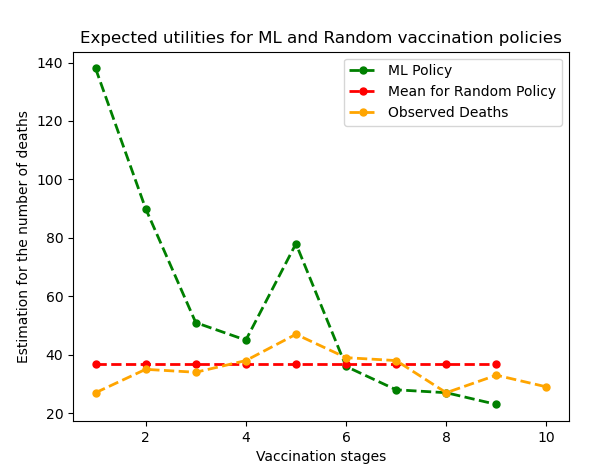
\includegraphics[width=8cm]{line_plot.png}
    \centering
    \caption{A simulation of a 10 vaccination stages where decisions were selected from the following policy: Random, Random, Random, Random, Random, Random, ML, ML, ML, ML.}
    \label{fig:1}
\end{figure}

The result of our vaccination decision process is that the machine learning model must first learn sufficiently well to make predictions which are better than a random vaccination policy. When we test the policy update pipeline, we observe that for the first six iterations, the model does not produce an action set which results in an expected utility better than the mean expected utility of the random policy (that is, the number of deaths predicted as a result of the model's estimation is higher than the expected deaths under the random policy). However, as the model is able to be trained on more data, the number of expected deaths from the learned actions drops to a level where we expect fewer deaths when the model suggested actions are taken. As shown in Figure \ref{fig:1}, after 6 vaccination stages the expected number of deaths from the ML Policy is lower than the average from the Random Policy (calculated over 6 stages of Random Policy observations). We are then able to switch to using the learned model to determine our action rather than the random policy and vaccinate the population according to the model output. Through this process, we observe that the expected utility very closely matches the observed outcomes for the machine learning model, indicating that the model has fit the data appropriately and the estimated number of deaths from our ML policy is close to the true outcome (orange dashed line). 

\section{Reproducibility}
\label{chap:Reproducibility}

This project can be reproducible by the code stored at our GitHub repository \href{https://github.com/fabiorodp/IN_STK5000_Adaptive_methods_for_data_based_decision_making/tree/main/project2}{https://github.com/fabiorodp/ IN\_STK5000\_Adaptive\_methods\_for\_data\_based\_decision\_making/tree/main/project2}. The results are achieved again with a high degree of reliability when the methodologies are replicated by the file \textbf{\textit{main\_part\_a1.py}} and \textbf{\textit{main\_part\_a2.py}}.

\section{Privacy}

In this section, we address the issue of privacy in the construction of our vaccination policy. As this database contains potentially sensitive information which may allow identification of the individuals described in it, we discuss several questions of privacy protection of the data and describe the methods by which we attempt to minimise the risk of data exposure.

\begin{itemize}
\item \textbf{\textit{Does the existence of this database raise any privacy concerns?}}

The database has several attributes that could be potentially important information that people would want to keep private. Most important among these is likely genetic data, which is highly sensitive and could potentially be used to find health conditions or susceptibility to health conditions. The age feature is also important as well, particularly because it is stored as a float, which suggests that this feature could be used to determine an exact date of birth. As dates of birth are frequently used for identity verification, this could pose a serious risk of identity theft to the individuals involved and therefore the resulting financial difficulties. Combined with gender this feature is also problematic, in consideration of the fact that as $87\%$ of Americans can be identified by birth date, gender and post code (see \textcolor{blue}{\cite{Dimitrakakis}}, p. 74), we can expect that similar conditions apply in all countries. Additionally, the vaccination status of individuals could also possibly be sensitive to certain individuals, as the revelation of this status could be the cause of interpersonal difficulties (e.g. bullying) among certain populations.  Furthermore, the income feature has potential to lead to similar outcomes if exposed. In particular, we may expect there is potential for making individuals with higher incomes more identifiable as targets for advertising or scams, and lower income individuals as targets for predatory lending or discrimination. Finally, comorbidities are an issue of significant privacy concern, as the release of an individuals medical conditions can similarly make them identifiable for targeted advertising as well as potential discrimination from employers, insurers, or others on the basis of these conditions.

\item \textbf{\textit{If the database was secret, but your analysis public, how would that affect privacy?}}

If the database was secret while the analysis was public, the privacy of the data would be more strongly protected. This scenario would prevent the direct use of the data by malicious actors for their own analysis of the population (perhaps attempting to de-anonymize the data by identifying the individuals from attributes). This setup of keeping the data secret would, however, compromise the ability of other researchers to reproduce the analysis that we present. One solution for this would be to create a synthetic data-set based on the distributions and attributes of the real data. This does rely on trust that the synthetic data is generated appropriately and conforms to the structure of the real data, but provides the opportunity for other researchers to apply the methods presented in the analysis. Moreover, it would be safer to only release real features which were most important in the original analysis, so that features which are not relevant to the task at hand cannot be used at all, reducing the exposition of the entire real data. Alternatively, it would also be possible to allow access to real data only through an API which implements a Differential Privacy Algorithm (e.g. \textit{$\epsilon$-differential privacy, $T$-fold adaptive composition, the Laplace mechanism, the exponential mechanism}, and other) under user registration and term of responsibility. It is essential to say that these differential privacy techniques are connected to learning theory and reproducibility (see \textcolor{blue}{\cite{Dimitrakakis}}, p. 79), therefore preferable than other simpler privacy approaches.

%Laplace mechanism, E_pi(a|x) should be similar to f(x) on the data.

\item[(A)] \textbf{\textit{Explain how you would protect the data of the people in the training set.}}
%Laplace mechanism

The first way in which we protect the privacy of the people in the training set is to create our Trusted Curator object. As described in Section \ref{adaptive_procedure}, we create an object to manage access to the data, where username and password credentials are required to draw a sample from the data. This ensures that we can limit access to this database to trusted researchers or other individuals who contact the holders of the data to obtain access credentials. 

There are certain other transformations we can apply to the data in order to make it less individually identifiable. For instance, we can begin by looking at one of the more straightforward privacy-preserving applications, namely k-anonymity, because there are some \textit{quasi-identifiers} in our database that are particularly sensitive, e.g., age, gender, income. The first transformation we make is to transform the age variable from a float to an integer. This could be taken even further by transforming each to a range (buckets comprising for instance decades like 30-39, 40-49 and so on), however we do not implement this for our model. Similarly, this could be done for the income feature by bucketing income into different brackets rather than storing the exact number. This would impair calculating averages on these features, but it would strongly reduce how distinguishable the individuals in the data are. Another approach we can take is to use a \textit{Laplace Mechanism} which adds noise $\omega \sim Laplace$ to the sensitive attribute. This is the local privacy approach to \textit{Differential Privacy} on the Income feature, and so any functions applied to this feature (for instance calculating an average, or use in an estimator) will also be differentially private.

We therefore use three approaches within our Trusted Curator to protect the privacy of the people in the training set. The first, as mentioned previously is to transform the age feature from a float to an integer. This will then conceal the exact date of birth of the individual record. The second transformation we apply to the data is a \textit{Randomized Response} mechanism over the \textit{Gender} attribute. The mechanism draws a number from a $Bernoulli$ distribution (i.e. flips a fair coin) and if the number is greater than $0.5$, we again draw a number $n \in \{0, 1\}$ and insert this value in place of the original gender attribute (it may be the same as before). Therefore some number of the gender attributes will be flipped in the data. The third transformation to the data is to use the \textit{Laplace Mechanism} as described in the previous paragraph to add noise to the Income attribute. The advantage of applying a differential privacy method to this attribute is that any functions calculated from this attribute will also be differentially private.

\item[(B)] \textbf{\textit{Explain how would protect the data of the people that obtain treatment.}}

As an additional measure besides our Trusted Curator, we apply another differential privacy algorithm when calculating the utility of our vaccination policy. When we calculate the effect of our vaccination policy to assess the efficacy of our actions $A$, we observe the outcomes $Y$ from the vaccination group and use the number of deaths in this group (i.e. a sum) to evaluate our policy. This is a summary statistic over the population who received vaccinations, and so when calculating this from our data, we are able to make use of differential privacy algorithms in order to protect the privacy of the people who are given vaccination with outcomes $Y$. The use of such an algorithm when we calculate the statistic necessary to evaluate our policy will allow us to estimate the efficacy of our policy while hiding the data to a degree of privacy defined by $\epsilon$. As described previously with respect to the Laplace Mechanism, a differentially private result ensures that any functions calculated using this attribute will then be differentially private. 

The primary mechanism to protect the data of the people who are vaccinated in our policy is therefore an \textit{Exponential Mechanism} applied to the \textit{Death} column in our output $Y$. In the Exponential Mechanism, we have two variables which influence the modification of the data: The sensitivity of our utility function $\mathbb{L}(U)$ and $\epsilon$, which defines the degree of trade-off between accuracy of the calculation and preservation of privacy. The sensitivity of a function is defined as $\mathbb{L}(U)\stackrel{\Delta}{=}\underset{xNx}{\sup}|U(q,a,x) - U(q,a,x')|$, where two sets of data $x$ and $x'$ which differ only by one element. This means that here our sensitivity is merely $\mathbb{L}(U) = 1$, as the values in our data are binary, and thus a difference of one element in summing the deaths will be a difference of $1$. We are then free to choose the parameter $\epsilon$ and observe the effects on the utility of the ML policy.

\item[(C)] \textbf{\textit{Implement a private decision making mechanism for (b).}}

As described in (B), we apply an \textit{Exponential Mechanism} to the \textit{Death} column in our output $Y$. In implementation this is to say that we calculate the probability of survival in the population, and repopulate the values of the column according to this probability distribution modified by our privacy guarantee $\epsilon$. This modification to the data therefore affects the calculation of the utility of our ML policy, and thus the actions we decide to take in the population. Our choice of $\epsilon$ is therefore of great importance not just due to the effect on how well the privacy of the data is preserved, but also because the effect of better preserving privacy may cause our policy to make a less accurate decision in our vaccination ML policy. Choosing the wrong value of $\epsilon$ result in an ineffective policy which results in a higher number of deaths as a consequence. It is therefore crucial to understand the loss in utility of our policy for different values of $\epsilon$ in our privacy preserving decision making process.

%In the Exponential Mechanism, we have two variables which influence the modification of the data: The sensitivity of our utility function $\mathbb{L}(U)$ and $\epsilon$, which defines the degree of trade-off between accuracy of the calculation and preservation of privacy. The sensitivity of a function is defined as $\mathbb{L}(U)\stackrel{\Delta}{=}\underset{xNx}{\sup}|U(q,a,x) - U(q,a,x')|$, where two sets of data $x$ and $x'$ which differ only by one element. This means that here our sensitivity is merely $\mathbb{L}(U) = 1$, as the values in our data are binary, and thus a difference of one element in summing the deaths will be a difference of $1$. We are then free to choose the parameter $\epsilon$ and observe the effects on the utility of the policy.

%In order to protect privacy of the vaccination group as described in (B), we are able to use the \textit{Laplace Mechanism}, which adds randomly generated noise to the calculation of the rate of deaths in the population, drawn from a Laplace distribution. When calculating $\hat{p} = \frac{d}{T}$, $d$ is defined as the sum $f(x)$ of deaths in the population. Instead of calculating this sum $d = f(x)$, we instead take $d = f(x) + \omega$ where $\omega \sim Laplace$. The parameter $\lambda$ of this Laplace distribution is defined by our privacy parameter $\epsilon$ and the sensitivity $\mathbb{L}(U) = 1$ (by definition of the sensitivity\cite{Dimitrakakis} such that $\lambda = \frac{\mathbb{L}}{n\epsilon}$ where $n$ is the number of individuals in our sample.

\item[(D)] \textbf{\textit{Estimate the amount of loss in utility as you change the privacy guarantee.}}

When using the \textit{Exponential Mechanism} to preserve privacy in the vaccination outcomes, we define our parameter $\epsilon$. For this reason, we test our policy under differing values for $\epsilon$ and compare the resulting utility value of our policy between these values as well as without the privacy guarantee (our original results above). We wish to observe the difference in policy outcomes when different parameter values for $\epsilon$ are applied to the data.


\begin{table}[hbpt]
\centering
\begin{tabular}{||c || c | c | c | c | c | c | c | c | c | c || c ||} 
\hline
 $\epsilon$ & \textbf{1} & \textbf{2} & \textbf{3} & \textbf{4}  & \textbf{5} & \textbf{6} & \textbf{7} & \textbf{8} & \textbf{9} & \textbf{Mean} & \textbf{loss} \\[0.5ex] 
 \hline\hline
 real & 140 & 90 & 55 & 45 & 80 & 38 & 30 & 30 & 25 & 59 & 0\\
 \hline
 0.5 & 166 & 125 & 179 & 138 & 91 & 72 & 58 & 65 & 43 & 104 & 45\\
 \hline
 \textbf{2.5} & \textbf{113} & \textbf{131} & \textbf{68} & \textbf{44} & \textbf{35} & \textbf{13} & \textbf{30} & \textbf{12} & \textbf{16} & \textbf{51} & \textbf{8}\\ 
 \hline
 4.5 & 86 & 222 & 157 & 91 & 59 & 51 & 54 & 77 & 34 & 92 & 33\\ 
 \hline
 6.5 & 412 & 291 & 105 & 74 & 166 & 72 & 24 & 105 & 87 & 149 & 90\\
 \hline
 8.5 & 115 & 253 & 139 & 106 & 144 & 98 & 53 & 43 & 75 & 114 & 55\\
 \hline
 10.5 & 216 & 233 & 109 & 190 & 135 & 117 & 55 & 36 & 64 & 128 & 69\\
 \hline
 12.5 & 545 & 123 & 229 & 368 & 60 & 208 & 106 & 70 & 70 & 198 & 139\\ [1ex] 
 \hline
\end{tabular}
\label{tab:utility-differences}
\caption{Expected utility by vaccination stage for Non-private calculation (real) and values of $\epsilon$. The 'loss' column is the absolute value of the difference between the Mean of the non-private calculation and the $\epsilon$-differentially private calculation of that row.}
\end{table}

\begin{figure}[H]
    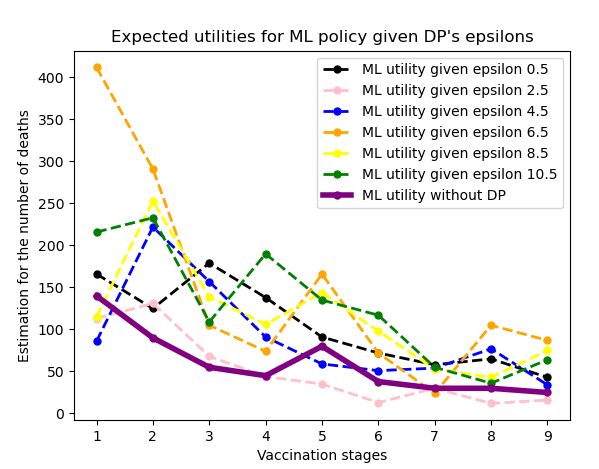
\includegraphics[width=12cm]{line_plot2.png}
    \centering
    \caption{Expected utility of the ML policy under a given DP's epsilon.}
    \label{fig:2}
\end{figure}

The epsilon value which most closely tracks the performance of our model is $\epsilon = 2.5$. This may indicate that we can choose the value of $\epsilon = 2.5$ and achieve comparable results to our model without the privacy guarantee. However, as this is an approximation over randomly sampled data from the population, the estimates are only a rough reflection of the difference in policy utility when the privacy guarantee is applied. More significantly, the results here may also reflect downstream results of the methods used on the training data to preserve privacy.

%The expected utility $\mathbb{E}(U)=T \cdot \hat{p}$ where $\hat{p} = \frac{d}{T}$. As discussed in (C), our privacy guarantee modifies $d$ to be defined as $d = f(x) + \omega$ (a centralized model of privacy, calculated by adding noise after the sum). The loss in utility from the privacy guarantee can be expressed as the difference between $\mathbb{E}(U)=T \cdot \frac{d}{T}$ and $\mathbb{E}(U')=T \cdot \frac{f(x) + \omega}{T}$ where $U'$ is the privacy preserving utility function utilizing the Laplace Mechanism.

%$(T \cdot \frac{d}{T}) - (T \cdot \frac{f(x) + \omega}{T})$
%.

%$(d) - (f(x) + \omega)$
%.

%$\omega$

%Thus, the loss of utility in our model is equal to the noise generated by the Laplace distribution. As $\mathbb{L} = 1$ by definition (the sum function differs by only $1$ between two sets of data $x$ and $x'$ where $1$ element differs, and the elements $e \in \{0, 1\}$), this means that our choice of $\epsilon$ entirely determines $\omega \sim Laplace$. The smaller $\epsilon$ is, the larger the parameter $\lambda$ of $Laplace$ is, and thus the stronger the noise effect, tending towards infinite loss of utility as $\epsilon$ approaches $0$. For example, if we assume $\epsilon = 0.5$ and the sample size each time we calculate our sum is $n = 10,000$ we then have $\lambda = \frac{1}{(0.5)(10,000)} = \frac{1}{5,000}$ as our parameter to the Laplace Mechanism. Under the centralised privacy model, the variance of the Laplace Mechanism is $2(\frac{\mathbb{L}}{\epsilon n})^2$, so with $\epsilon = 0.5$ we have a variance of $1 \times 10^-8$, whereas if $\epsilon=0.2$ then the variance is $5 \times 10^-7$.

\end{itemize}

\printbibliography
\end{document}
